\documentclass{article}

\usepackage{physics} % Handy shortcuts like \pdv, \dd and much more
\usepackage[top=3cm]{geometry} % smaller margins, can be adjusted if given arguments
\usepackage{siunitx} % the \si environment for units
\usepackage{mathtools} % The dcases environment, prettier than just cases
\usepackage{tikz} % For drawing picures
\usepackage{wrapfig} % Wrapping text around figures


\title{Exercise 4 - TFY4345 Classical Mechanics}
\date{2020}

\begin{document}
    \maketitle
    \section{Mathematical pendulum in accelerated motion} 
        \begin{wrapfigure}{2}{0.2\textwidth}
            \vspace{-1cm}
            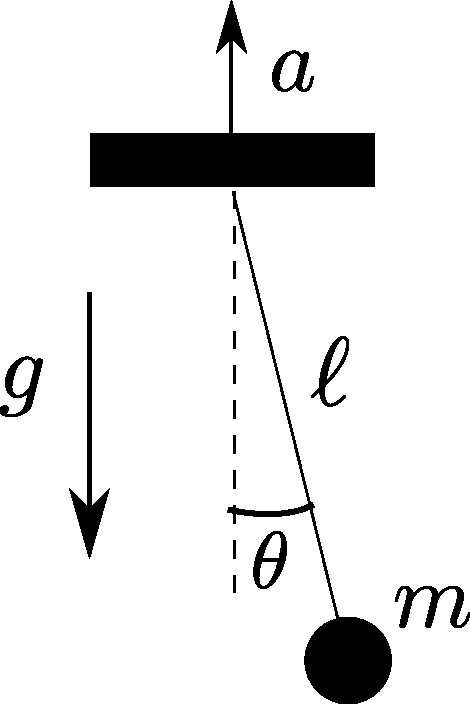
\includegraphics[width=0.2\textwidth]{figures/figure_1.pdf}
            \vspace{-2cm}
        \end{wrapfigure}
        The pendulum is lifted with a constant acceleration $a$. Derive the Hamiltonian and Hamilton's equations of motion. Does the relation $H = E$ hold, and is $H$ a constant of motion?

    \section{Spherically symmetrical potential}
        A moving particle experience a potential 
        \begin{equation*}
            V(r) = -\frac{k}{r}.
        \end{equation*}
        Determine the Hamiltonian and Hamilton's equations of motion using spherical coordinates.

    \section{Earth's orbit}
        Assume the Earth's orbit to be circular and that the Sun's mass suddenly decreases to one half. What orbit will Earth then have? Will it escape from the solar system? Use the equations for eccentricity.

    \section{Einsteins correction}
        A single particle with mass $m$ moves in a central force field, and experiences a force 
        \begin{equation*}
            f(r) = -\frac{k}{r^2} + \frac{\beta}{r^3},
        \end{equation*}
        where $\beta$ is a constant. This is an extension of the original Kepler problem, to include Einstein's correction from the general thoery of relativity. Show that the resulting trajectory can be written in the form 
        \begin{equation*}
            \frac{p}{r} = 1 + \varepsilon \cos(\gamma \theta),
        \end{equation*}
        which gives an ellipse for $\gamma = 1$, and precession of the orbit otherwise. For Mercury the value of $\beta$ is $43 \, \mathrm{arc}\, \mathrm{seconds}/\mathrm{century}$. Find the expression for $\varepsilon, p$ and $\gamma$. \\ \\
        (Hint 1: Start from the related integral in the original Kepler problem as discussed in the lecture notes and course book.) \\
        (Hint 2: Identify that $\gamma² = 1 + \beta m / \ell^2$ before integration, and use it later in the definitions of $\varepsilon$ and $p$.)

\end{document}

